\documentclass{article} 
    %\usepackage[margin=0.8in]{geometry}
    %\usepackage[parfill]{parskip}
    \usepackage[utf8]{inputenc}
    \usepackage{graphicx}
    \usepackage{siunitx}
    \usepackage{amsmath}
    \usepackage{listings}
    \usepackage{color}


% Letternumbering
\renewcommand{\thesection}{Part \Alph{section}} 

\title{Artificial Intelligence Methods, exercise 4}
\author{Rendell Cale}
\date{\today}

\begin{document}

\maketitle

\section{}
\begin{centering}
	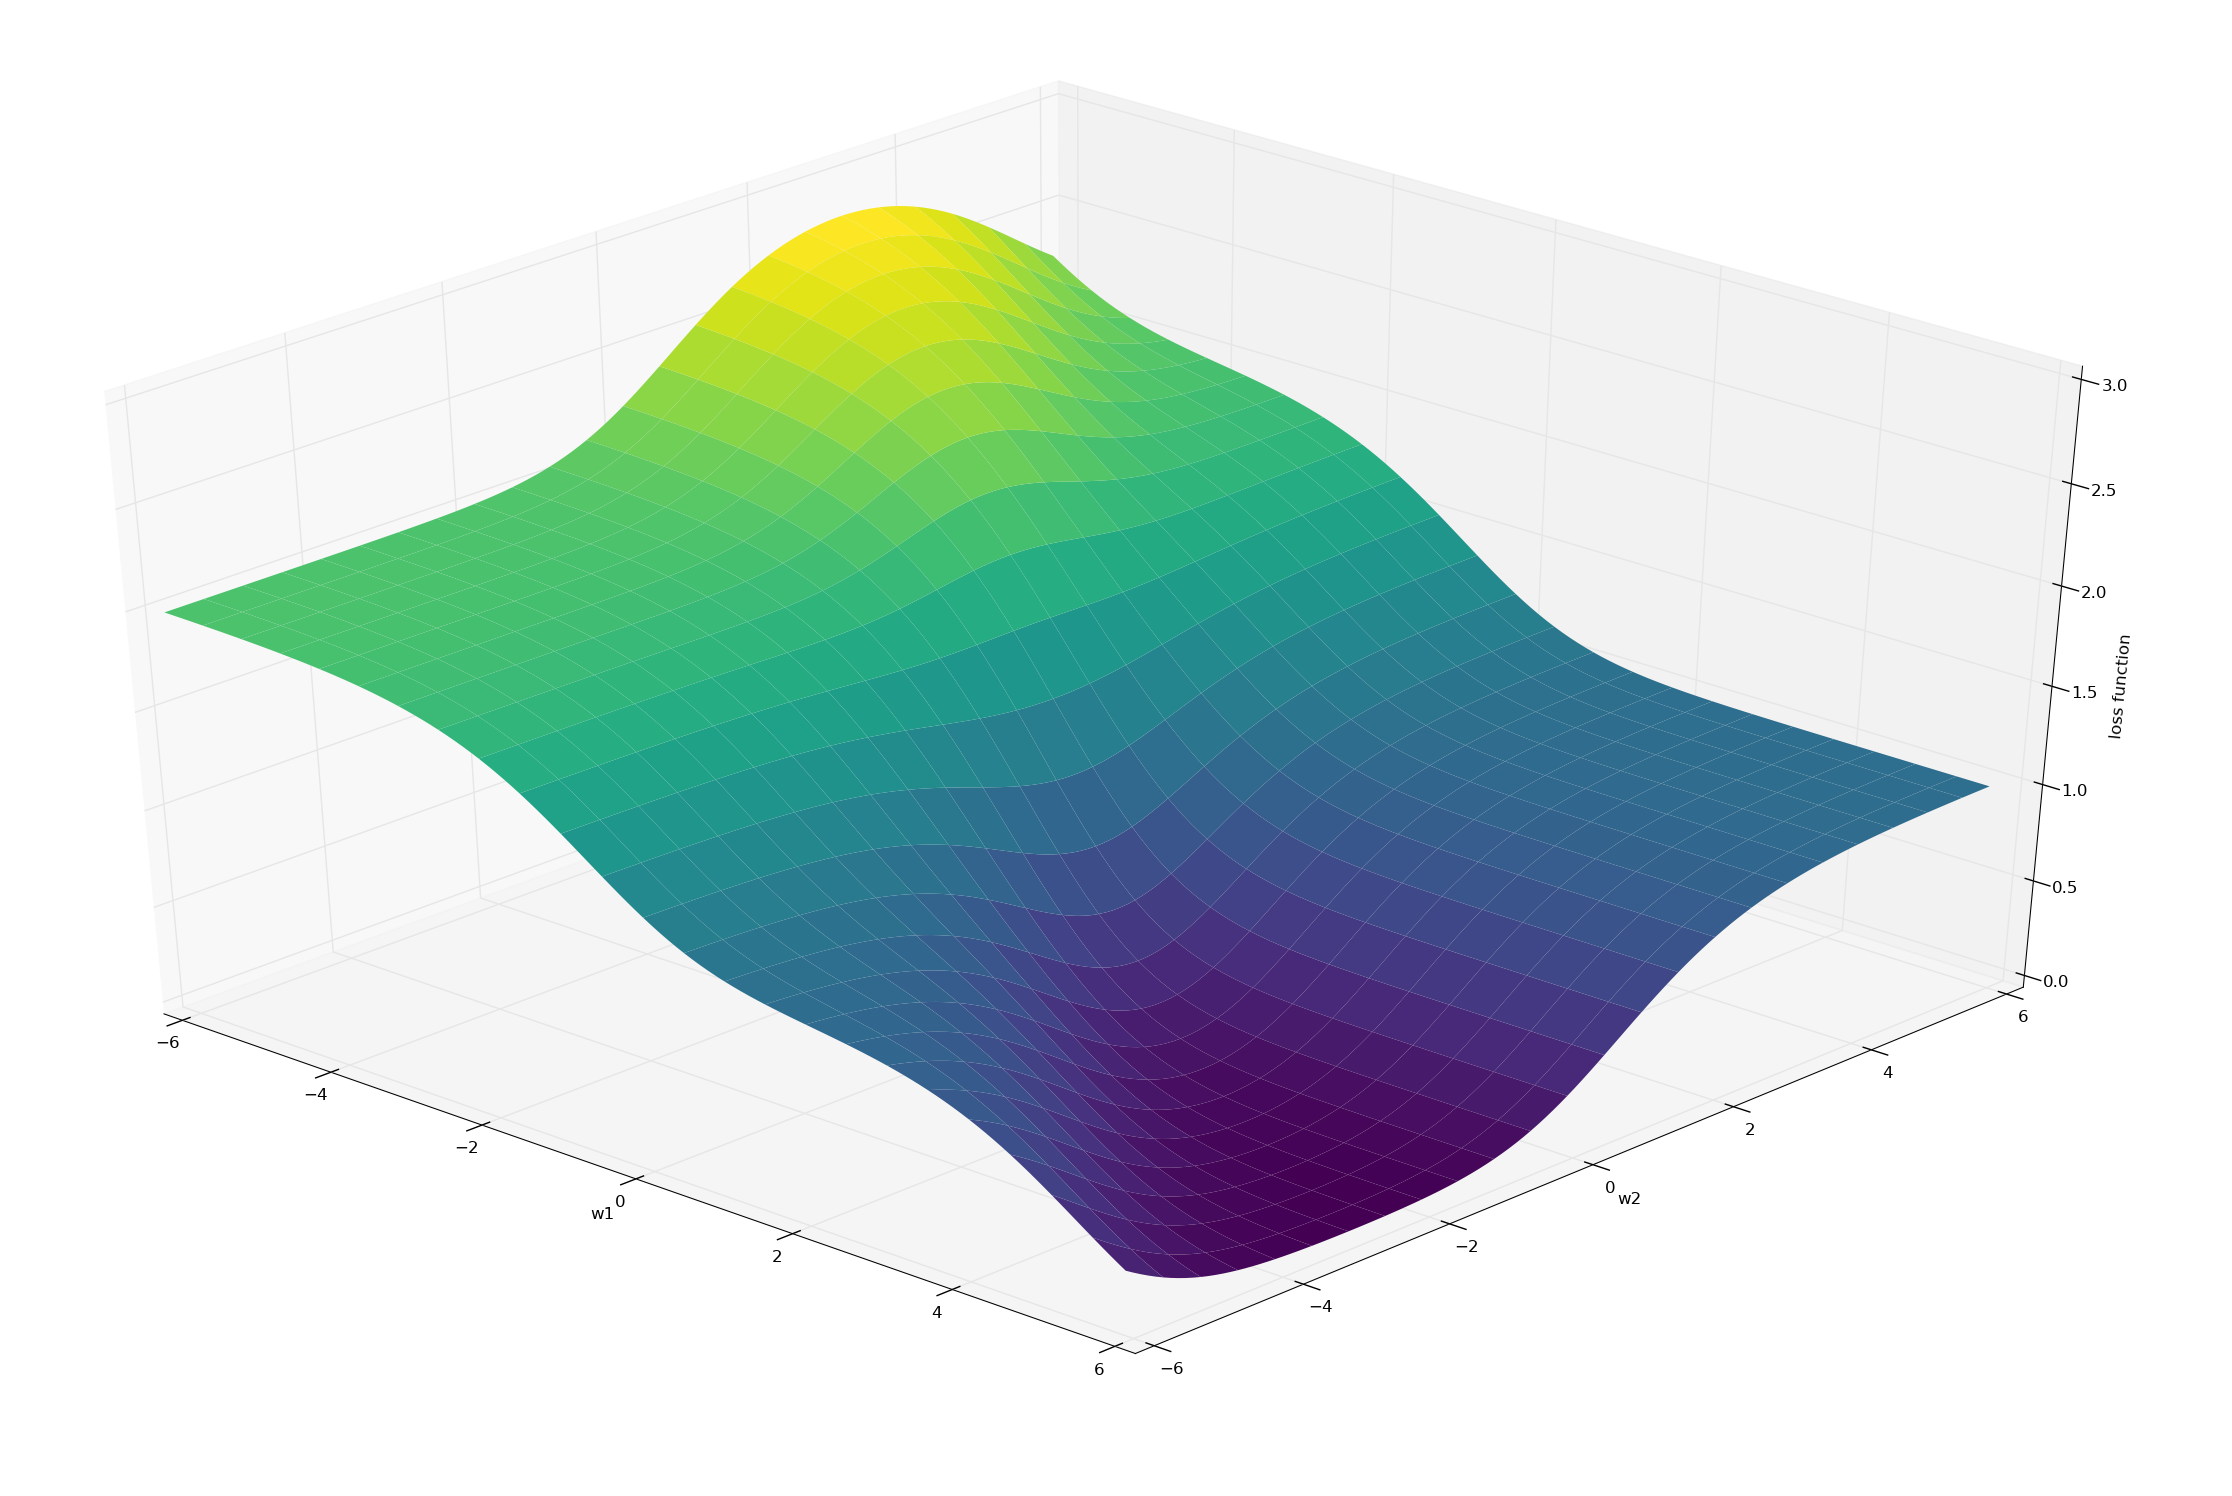
\includegraphics[width=\linewidth]{exercise4_task1.png}
\end{centering}

From the plot it does not seem that there is a definite lowest point, but rather that the function decreases monotonically toward zero in the as $w=(w_1,w_2)=(w, -w)$ and $w \rightarrow \infty$. 

\subsection{}

\subsection{}
Using the definitions for $\sigma(w,x)$ and $L_{simple}(w)$,
\begin{align}
	\sigma(w,x) &= \frac{1}{1 + e^{-w^Tx}} \\
	L_{simple} &= \left[ \sigma(w,[1,0]) - 1 \right]^2 + \sigma(w,[0,1])^2 + \left[ \sigma(w,[1,1]) - 1 \right]^2,
\end{align}
we can compute the gradient of $L_{simple}$, $\nabla_w L_{simple}$.

We begin by writing out the expression using $w = [w_1, w_2]^T$.

\begin{align}
	L_{simple} &= \left[ \frac{1}{1 + e^{-w_1}} - 1 \right]^2 + \left[ \frac{1}{1 + e^{-w_2}} \right]^2 + \left[ \frac{1}{1 + e^{-w_1 - w_2}} - 1 \right]^2 \\
	&= \left[ \sigma(w_1) - 1 \right]^2 + \sigma(w_2)^2 + \left[ \sigma(w_1 + w_2) - 1 \right]^2.
\end{align}

It is quite well known that
\begin{equation}
	\frac{\partial \sigma(x)}{\partial x} = \sigma(x) (1 - \sigma(x))
\end{equation}

Using this and the chain rule, we find that
\begin{align}
	\frac{\partial L_{simple}}{\partial w_1}(w) = 2 \left[ \sigma(w_1) - 1 \right]  \frac{\partial \sigma(w_1)}{\partial w_1}  + 2 \left[ \sigma(w_1 + w_2) - 1 \right] \frac{\partial \sigma(w_1 + w_2)}{\partial w_1} \\
	= 2 (\sigma(w_1) - 1)\sigma(w_1)(1 - \sigma(w_1)) + 2 (\sigma(w_1 + w_2) - 1) \sigma(w_1 + w_2)(1 - \sigma(w_1+w_2)) \\
	= -2 \left[ \sigma(w_1) - 1 \right]^2\sigma(w_1) -2 \left[ \sigma(w_1 + w_2) - 1 \right]^2\sigma(w_1 + w_2).
\end{align}

For $w_2$ we get
\begin{align}
	\frac{\partial L_{simple}}{\partial w_2}(w) &= 2\sigma(w_2)\sigma(w_2)(1 - \sigma(w_2)) + 2 \left[ \sigma(w_1 + w_2) - 1 \right] \sigma(w_1+w_2)(1 - \sigma(w_1 + w_2)) \\
	&= 2 \sigma(w_2)^2(1 - \sigma(w_2)) - 2 \sigma(w_1+w_2) \left[ \sigma(w_1+w_2) - 1 \right]^2.
\end{align}

\subsection{}
After implementing the update rule in Python, starting the weights at $(w_1,w_2) = (0,0)$, running it for $10000$ iterations and plotting the surface along with the search results for different $\eta$, I get:

\begin{centering}
	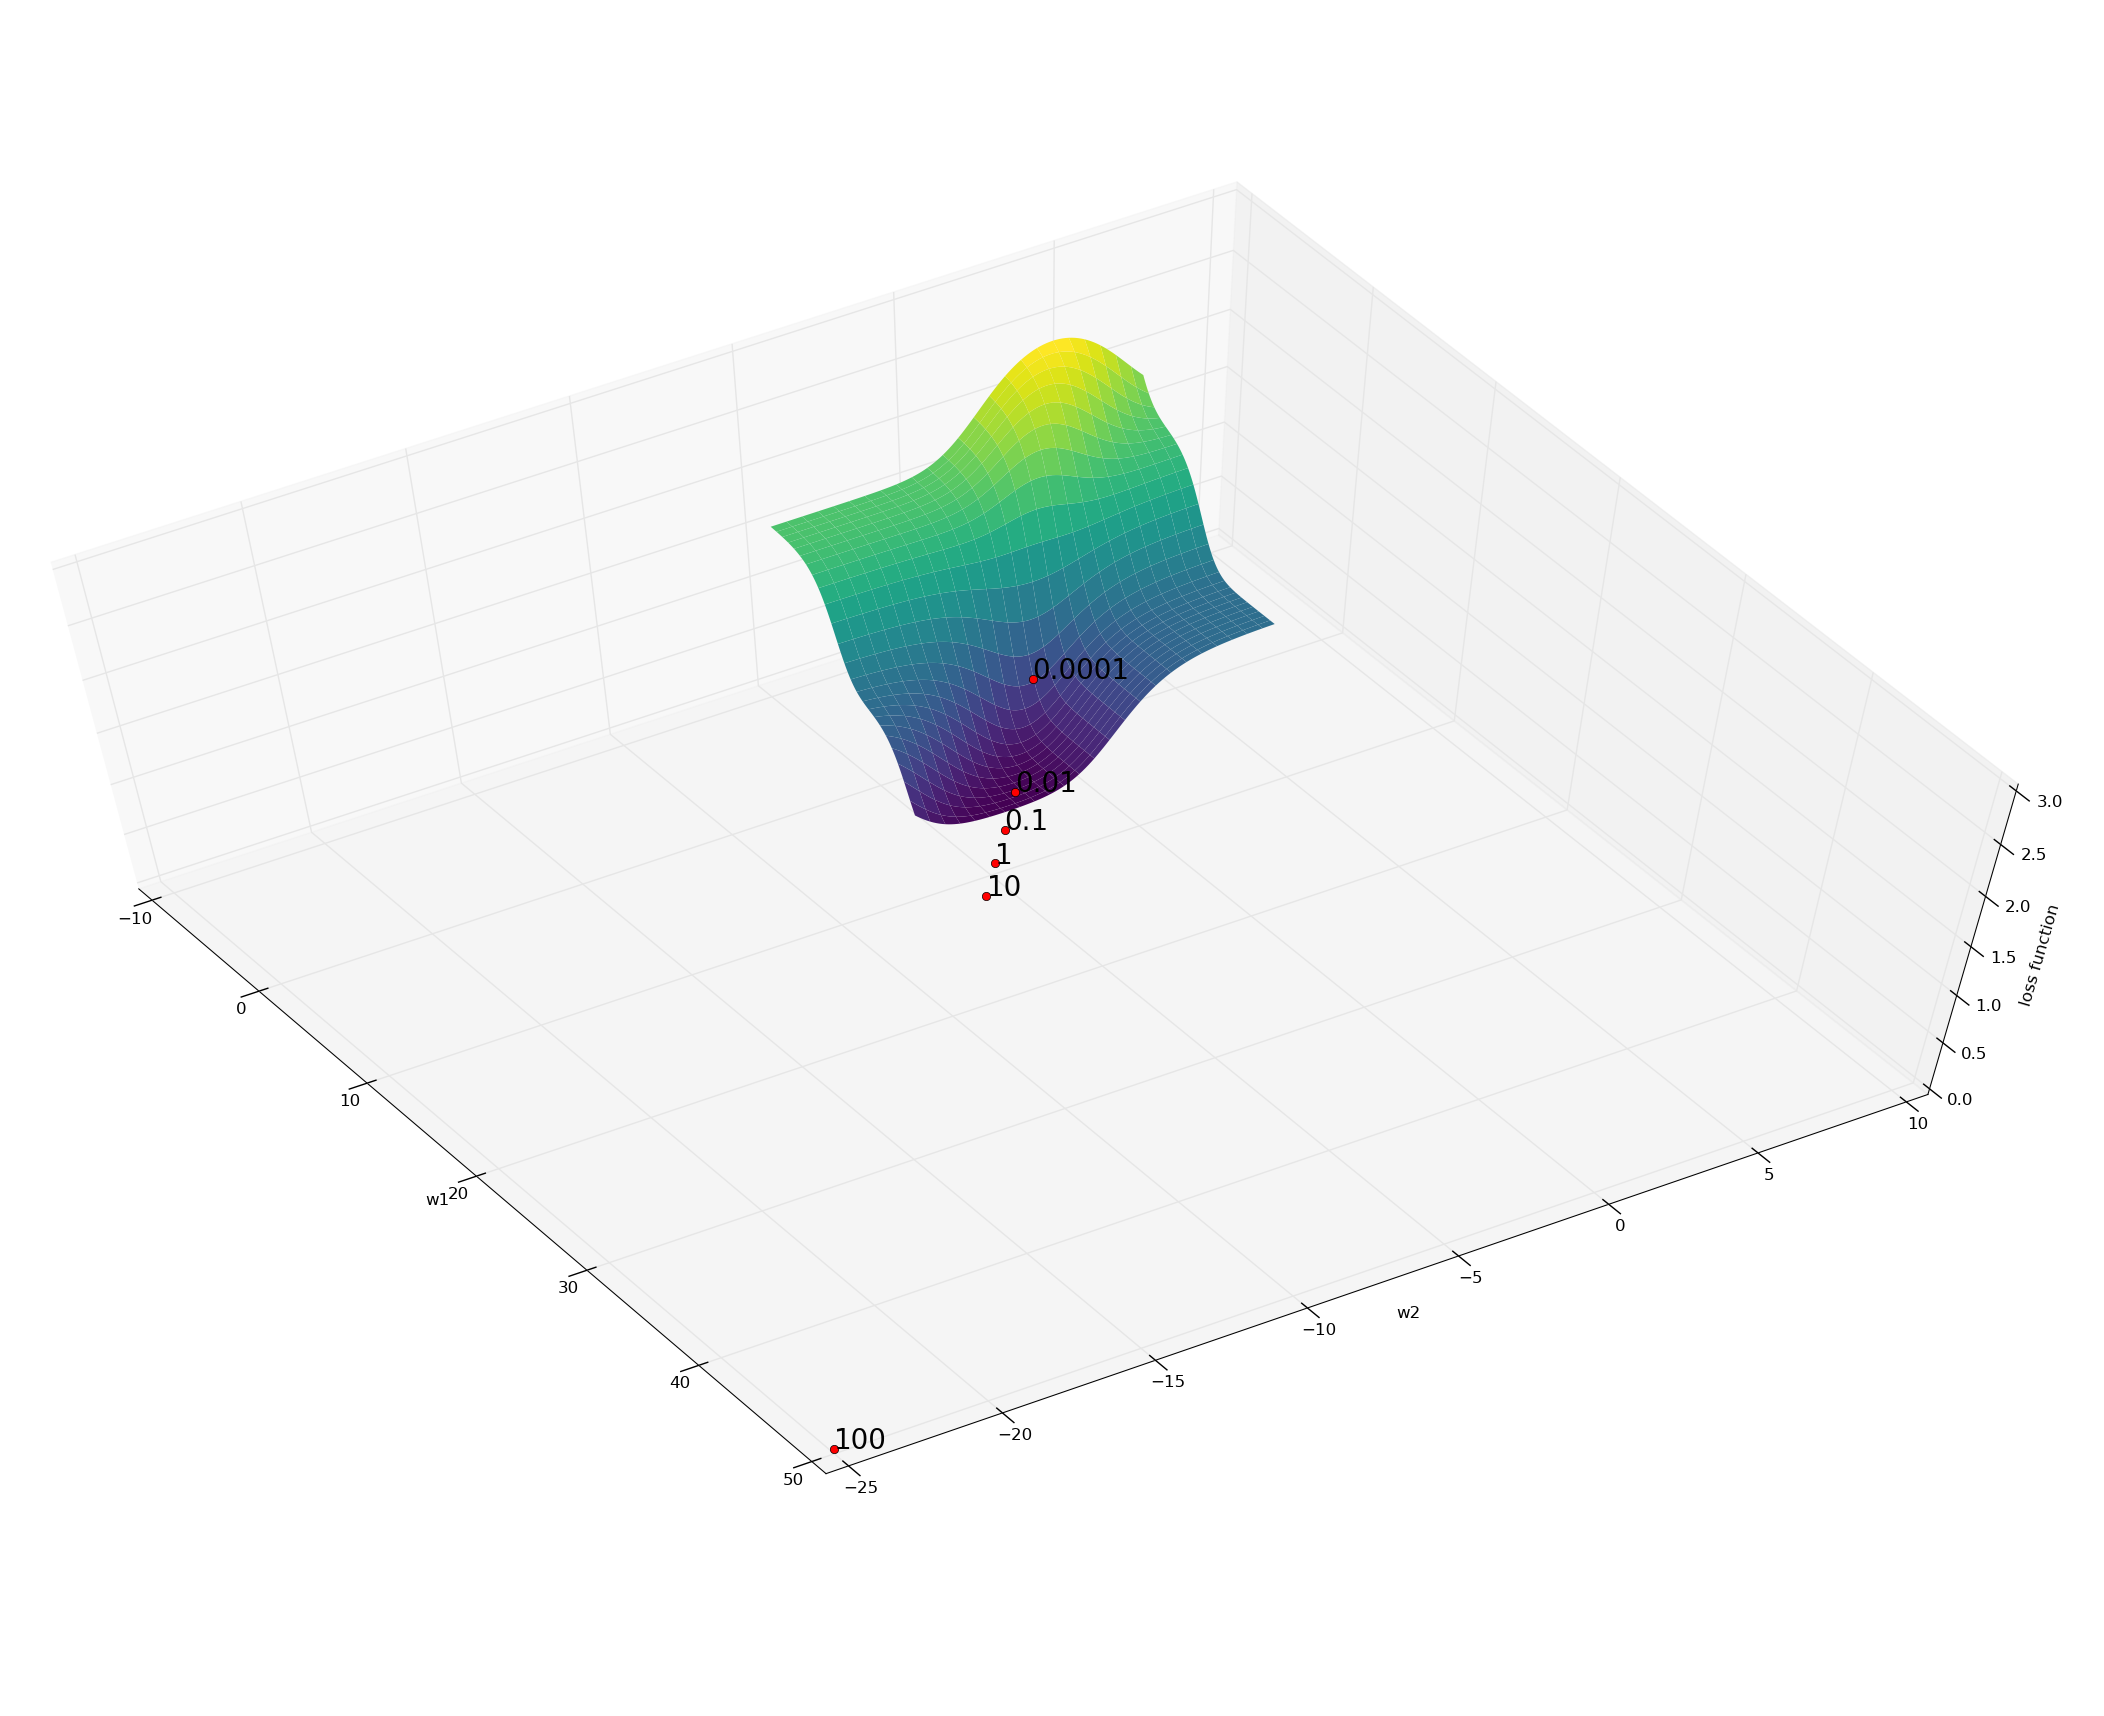
\includegraphics[width=\linewidth]{exercise4_task13.png}
\end{centering}

Notice in the plot that there is quite a big difference between the different choices of $\eta$. With $\eta = 100$ the weights ended up quite far away from the others, but actually the difference in the loss function values of the resulting points isn't that big when we compare $\eta = 100$ to $\eta = 0.01$. 
The function does decrease in the direction of $(w_1,w_2) = (\infty,-\infty)$, but is essentially constantly zero from quite early on. 

Another interesting thing we can see from this plot is that for $\eta=0.0001$, the loss function is significantly larger. This is probably since the sequence converges slower for small values of $\eta$. 



\end{document}

